%\documentclass{article}
%\usepackage{graphicx,subfigure}
%\begin{document}

\begin{figure}[!h]
  \centering
   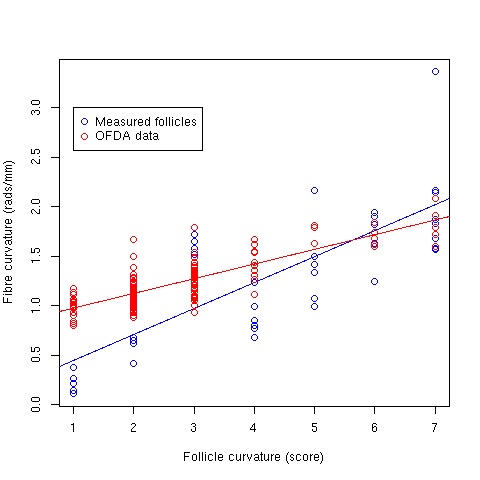
\includegraphics[width=0.9\textwidth]{ovly.png}
%  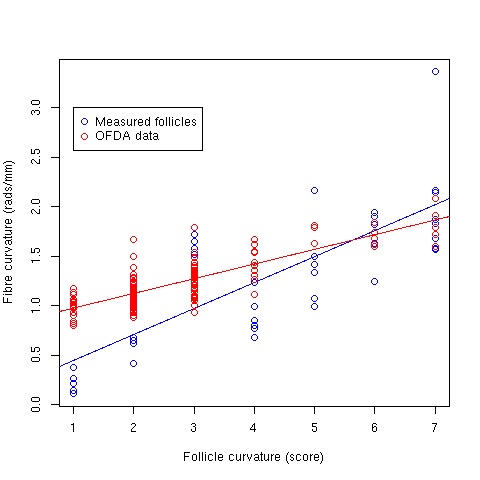
\includegraphics{ovly.png}
  \caption{Measured curvature of fibres in staples by OFDA technique for 159 sheep of   given follicle curvature score, superimposed on measured curvature of fibres in follicles. The two straight lines are orthogonal regression lines representing equations~\ref{eqn:in-follicle} and ~\ref{eqn:in-staple}.}
  \label{fig:ovly}
\end{figure}

%\end{document}

